\documentclass{report}
\usepackage{layout}
\usepackage[a4paper, total={5in,9in}]{geometry}
\usepackage[T1]{fontenc}
\usepackage{mathtools}
\usepackage{amsthm}
\usepackage[framemethod=TikZ]{mdframed}
\usepackage{amsmath}
\usepackage{amssymb}
\usepackage{cancel}
\usepackage[dvipsnames]{xcolor}
\usepackage{tikz}
\usepackage{tikz-cd}
\usepackage{pgfplots}
\pgfplotsset{compat=1.18}
\usepackage[many]{tcolorbox}
\usepackage{import}
\usepackage{pdfpages}
\usepackage{transparent}
\usepackage{enumitem}
\usepackage[colorlinks]{hyperref}
\usepackage{csvsimple}
\usepackage{listings}

\newcommand*{\sminus}{\raisebox{1.3pt}{$\smallsetminus$}}

\newcommand*{\transp}[2][-3mu]{\ensuremath{\mskip1mu\prescript{\smash{\mathrm t\mkern#1}}{}{\mathstrut#2}}}%

% newcommand for span with langle and rangle around
\newcommand{\Span}[1]{{\left\langle#1\right\rangle}}

\newcommand{\incfig}[2][1]{%
    \def\svgwidth{#1\columnwidth}
    \import{./figures/}{#2.pdf_tex}
}

\pdfsuppresswarningpagegroup=1

\newcounter{theo}[section]\setcounter{theo}{0}
\renewcommand{\thetheo}{\arabic{section}.\arabic{theo}}

\newcounter{excounter}[section]\setcounter{excounter}{0}
\renewcommand{\theexcounter}{\arabic{section}.\arabic{excounter}}

\numberwithin{equation}{section}

\newenvironment{theorem}[1][]{
    \refstepcounter{theo}
     \ifstrempty{#1}
    {\mdfsetup{
        frametitle={
            \tikz[baseline=(current bounding box.east),outer sep=0pt]
            \node[anchor=east,rectangle,fill=blue!20,rounded corners=5pt]
            {\strut Teorema~\thetheo};}
        }
    }{\mdfsetup{
        frametitle={
            \tikz[baseline=(current bounding box.east),outer sep=0pt]
            \node[anchor=east,rectangle,fill=blue!20,rounded corners=5pt]
            {\strut Teorema~\thetheo:~#1};}
        }
    }
    \mdfsetup{
        roundcorner=10pt,
        innertopmargin=10pt,linecolor=blue!20,
        linewidth=2pt,topline=true,
        frametitleaboveskip=\dimexpr-\ht\strutbox\relax,
        % nobreak=false
    }
\begin{mdframed}[]\relax}{
\end{mdframed}}
\newtcolorbox[auto counter, number within=section]{definition}[2][]{
    colframe=violet!0,
    coltitle=violet, % Title text color
    fonttitle=\bfseries, % Title font
    title={Definizione~\thetcbcounter:~#2}, % Title format
    sharp corners, % Less rounded corners
    boxrule=0pt, % Line width of the box frame
    toptitle=1mm, % Distance from top to title
    bottomtitle=1mm, % Distance from title to box content
    colbacktitle=violet!5, % Background color of the title bar
    left=0mm, right=0mm, top=1mm, bottom=1mm, % Padding around content
    enhanced, % Enable advanced options
    before skip=10pt, % Space before the box
    after skip=10pt, % Space after the box
    breakable, % Allow box to split across pages
    colback=violet!0,
    borderline west={2pt}{-5pt}{violet!40},
    #1
}

\newenvironment{lemmao}[1][]{
    \refstepcounter{theo}
     \ifstrempty{#1}
    {\mdfsetup{
        frametitle={
            \tikz[baseline=(current bounding box.east),outer sep=0pt]
            \node[anchor=east,rectangle,fill=green!20,rounded corners=5pt]
            {\strut Lemma~\thetheo};}
        }
    }{\mdfsetup{
        frametitle={
            \tikz[baseline=(current bounding box.east),outer sep=0pt]
            \node[anchor=east,rectangle,fill=green!20,rounded corners=5pt]
            {\strut Lemma~\thetheo:~#1};}
        }
    }
    \mdfsetup{
        roundcorner=10pt,
        innertopmargin=10pt,linecolor=green!20,
        linewidth=2pt,topline=true,
        frametitleaboveskip=\dimexpr-\ht\strutbox\relax,
        % nobreak=true
    }
\begin{mdframed}[]\relax}{
\end{mdframed}}

\theoremstyle{plain}
\newtheorem{lemma}[theo]{Lemma}
\newtheorem{corollary}{Corollario}[theo]
\newtheorem{proposition}[theo]{Proposizione}

\theoremstyle{definition}
\newtheorem{example}[excounter]{Esempio}

\theoremstyle{remark}
\newtheorem*{note}{Nota}
\newtheorem*{remark}{Osservazione}

\newtcolorbox{notebox}{
  colback=gray!10,
  colframe=black,
  arc=5pt,
  boxrule=1pt,
  left=15pt,
  right=15pt,
  top=15pt,
  bottom=15pt,
}

\DeclareRobustCommand{\rchi}{{\mathpalette\irchi\relax}} % beautiful chi
\newcommand{\irchi}[2]{\raisebox{\depth}{$#1\chi$}} % inner command, used by \rchi

\newtcolorbox[auto counter, number within=section]{eser}[1][]{
    colframe=black!0,
    coltitle=black!70, % Title text color
    fonttitle=\bfseries\sffamily, % Title font
    title={Esercizio~\thetcbcounter~#1}, % Title format
    sharp corners, % Less rounded corners
    boxrule=0pt, % Line width of the box frame
    toptitle=1mm, % Distance from top to title
    bottomtitle=1mm, % Distance from title to box content
    colbacktitle=black!5, % Background color of the title bar
    left=0mm, right=0mm, top=1mm, bottom=1mm, % Padding around content
    enhanced, % Enable advanced options
    before skip=10pt, % Space before the box
    after skip=10pt, % Space after the box
    breakable, % Allow box to split across pages
    colback=black!0,
    borderline west={1pt}{-5pt}{black!70},
}
\newcommand{\seminorm}[1]{\left\lvert\hspace{-1 pt}\left\lvert\hspace{-1 pt}\left\lvert#1\right\lvert\hspace{-1 pt}\right\lvert\hspace{-1 pt}\right\lvert}

\definecolor{codegreen}{rgb}{0,0.6,0}
\definecolor{codegray}{rgb}{0.5,0.5,0.5}
\definecolor{codepurple}{rgb}{0.58,0,0.82}
\definecolor{backcolour}{rgb}{0.95,0.95,0.92}
\lstdefinestyle{mystyle}{
    backgroundcolor=\color{backcolour},   
    commentstyle=\color{codegreen},
    keywordstyle=\color{magenta},
    numberstyle=\tiny\color{codegray},
    stringstyle=\color{codepurple},
    basicstyle=\ttfamily\footnotesize,
    breakatwhitespace=false,         
    breaklines=true,                 
    captionpos=b,                    
    keepspaces=true,                 
    numbers=left,                    
    numbersep=5pt,                  
    showspaces=false,                
    showstringspaces=false,
    showtabs=false,                  
    tabsize=2
}

\lstset{style=mystyle}

\title{Report Lab 1\\\small Experimental Physics for AI 2}
\author{G, C, D, O}
\date{First semester 2024 \-- 2025}

\begin{document}

\maketitle

\chapter{Measurement of the current-voltage characteristic of a resistor}
\chapter{Measurement of the current-voltage characteristic of a diode}
\section{Goal}
Now we want to measure the current-voltage characteristic of a diode, which
should not be linear. Indeed, according to Shockley's law, it is exponential:
\[
    I = I_0 \left( e^{\frac{qV}{gkT}} - 1 \right)
\]
where $I_0$ is the reverse saturation current, $q$ is the electron charge, \(k\)
is the Boltzmann constant, \(T\) is the temperature, and \(g\) is the diode
type-dependent constant. In this chapter we will try to verify this law.

Moreover for practical applications it's common practice to define the diode's
\emph{threshold voltage} as the voltage at which the diode starts conducting a
``significant'' current. We will try to measure this value as well.

\section{Method}
Using a similar setup as the one in part one, we recorded the measured values of
current at different voltages. The setup is shown in
figure~\ref{fig:setup-diode}, where the voltmeter is a handheld Fluke
multimeter and the ammeter is a Agilent bench multimeter.

\begin{figure}[ht]
    \centering
    \incfig[.45]{setup-diode}
    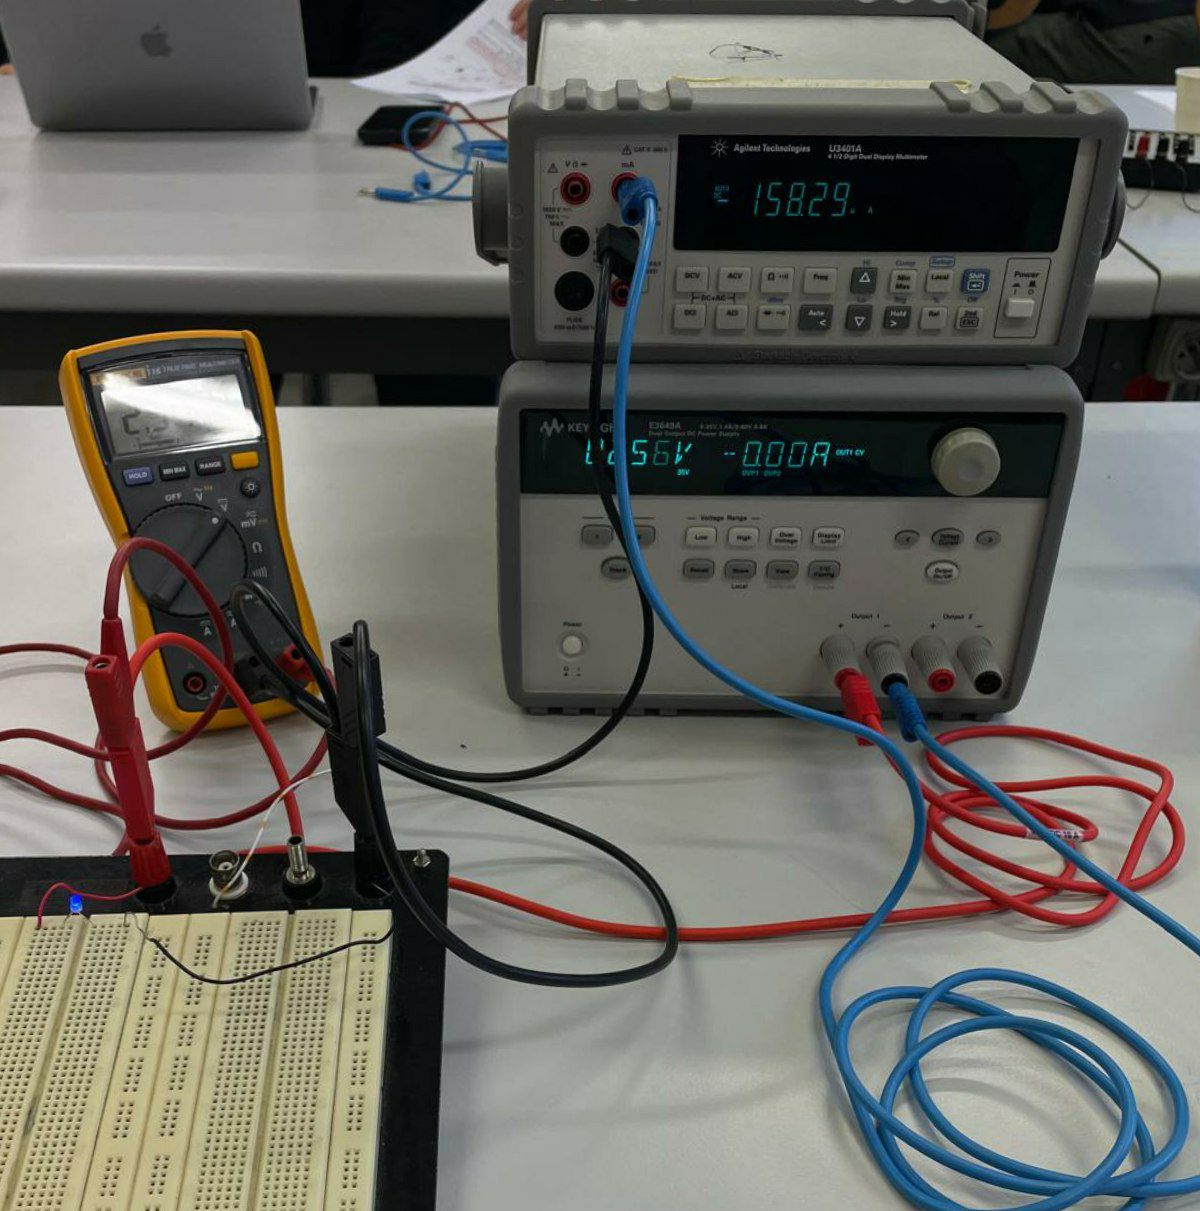
\includegraphics[width=.45\textwidth]{figures/setup.png}
    \caption{Setup of the diode experiment: on the left the diagram showing
    the circuit made, on the right a photo of the setup}\label{fig:setup-diode}
\end{figure}

Later, in section~\ref{sec:analysis}, we will perform various fits to the data to
verify the exponential relation and estimate the values of the parameters.

\section{Data}\label{sec:data}
The data we collected is shown in table and represented graphically in
figure~\ref{fig:diode-data}. The bench multimeter for the current measurements
had an accuracy of \(\pm 0.05\% + 0.05\mu A\) in the \(500 \mu A\) range; and
the handheld multimeter had an accuracy of \(\pm 0.5\% + 0.002V\) in the \(2 V\)
range.

\begin{figure}[ht]
	{\small
\begin{tabular}[ht]{ll|ll}
       \multicolumn{2}{l}{\bfseries Voltage (\(V\))} &
       \multicolumn{2}{l}{\bfseries Current (\(\mu A\))} \\
       \hline
       \csvreader[head to column names]{../data.csv}{}%
       {\Vdetapprox&$\pm$ \errVdet&\Idetapprox&$\pm$ \errIdet\\}
\end{tabular}}
\begin{tikzpicture}[baseline=(current bounding box.base), scale=.9]
    \begin{semilogyaxis} [
        table/col sep=comma,
        title = {Diode current-voltage data},
        xlabel = {Voltage (\(V\))},
        ylabel = {Current (\(\mu A\))},
        % xmin = 2,
        no markers,
    ]

    \addplot+ [
            only marks, mark size=.2pt,
            error bars/.cd,
                x dir = both, x explicit,
                y dir = both, y explicit,
        ] table [x=Vdetapprox, y=Idetapprox, x error=errVdet, y error=errIdet] {../data.csv};
    
    \end{semilogyaxis}
\end{tikzpicture}
       \caption{Data collected for the diode}\label{fig:diode-data}
   \end{figure}
   from the graph in figure~\ref{fig:diode-data} we can already see that after a
   certain voltage value (about 2.4) the graph follows accurately an exponential
   relationship, as expected. The previous values are very low in current and
   have a greater error. We will perform the analysis only on the part of the
   data which shows a clear exponential behavior, that is for voltages greater
   than \(2.399\) and currents greater than \(1.74\mu A\) (medium values).
   \section{Analysis}\label{sec:analysis}   

   \subsection{Shockley's law}
    We used the following approximation:
    \begin{equation}\label{eq:approx}
        \ln {(e^{x} - 1)} \approx x \quad \text{for } x \gg 1
    \end{equation}
    so that we could linearize the relationship as
    \[
        I = I_0 \left( e^{\frac{qV}{gkT}} - 1 \right) \approx I_0
        e^{\frac{qV}{gkT}} \implies \log I \approx \frac{q}{gkT} V + \log I_{0}
    \]
    Then we performed a linear regression on the data, with the errors on \(V\).
    We decided to keep the error only in the independent variable since it was
    much greater than the one in the dependent variable. 
   in \texttt{R} we ran the following commands:
\lstinputlisting[language=R, firstline=1, lastline=6]{../analysis.r}
   obtaining the following result:
   \begin{verbatim}
Coefficients:
            Estimate Std. Error t value Pr(>|t|)    
(Intercept)  -66.698      1.294  -51.55   <2e-16 ***
Vdetapprox    28.215      0.509   55.44   <2e-16 ***
---
Signif. codes:  0 ‘***’ 0.001 ‘**’ 0.01 ‘*’ 0.05 ‘.’ 0.1 ‘ ’ 1

Residual standard error: 44.5 on 19 degrees of freedom
Multiple R-squared:  0.9939, Adjusted R-squared:  0.9935 
F-statistic:  3073 on 1 and 19 DF,  p-value: < 2.2e-16  
   \end{verbatim}
   So we can very confidently say that the relation between the current and the
   voltage is exponential. The formula is then:
   \begin{align*}
       \log I_{0} = -67 \pm 1 &\implies I_{0} = 10^{-29} \pm 
       10^{-29} \mu A\\
       \frac{q}{gkT} = 28.2 \pm 0.5 &\implies g = \frac{38.6}{28.2} \mp
       \frac{0.5}{28.2^2} = 1.368 \pm 0.006\\
       I \approx 1e-29 e^{\frac{q}{kT} \cdot \frac{1}{1.368} \cdot V} &= 10^{-29}
       e^{28.2 V} \mu A
   \end{align*}
   (We did not take the measurement for the temperature, so actually 38.6 here
   should not obviously be a constant, but as we don't have the measurement, we
   considered it as such, consequently the error on \(g\) is much smaller than
   the one it should be).
   In figure~\ref{fig:fit} we can see in a graph the accuracy of the fit. Now we
   can justify the approximation~\eqref{eq:approx} as indeed for \(V \ge 2.4\)
   we clearly have that the exponent \(\frac{qV}{gkT} \ge 67.68 \gg 1\), more
   precisely, if \(f, g: [67.68, \infty)\) are respectively the functions \(x
   \mapsto \ln {(e^{x} - 1)}\) and \(x \mapsto x\) then
   \[
       \|f - g\|_{\infty} = |{(f - g)}{(67.68)}| \approx 4.05 \cdot 10^{-30}
   \]
   \paragraph{Chi-squared test} Finally, we performed a \(\rchi^2\)  test on the
   residuals of the fit to see if the errors were independent and normally
   distributed (assuming homoscedasticity), which is what we expect:
   \lstinputlisting[language=R, firstline=21]{../analysis.r}
   Which returns a p-value of \(0.65 > 0.05\), so we can't reject the null
   hypothesis that the errors are independent and the fit is good.
\begin{figure}
    \centering
\begin{tikzpicture}
    \begin{axis} [
        table/col sep=comma,
        title = {Diode current-voltage data},
        xlabel = {Voltage (\(V\))},
        ylabel = {Current (\(\mu A\))},
        xmin = 2.395, 
        ymax = 320,
        no markers,
        legend pos = north west,
    ]

    \addplot+ [
            only marks, mark size=1pt,
            error bars/.cd,
                x dir = both, x explicit,
                y dir = both, y explicit,
        ] table [x=Vdetapprox, y=Idetapprox, x error=errVdet, y error=errIdet] {../data.csv};
    \addlegendentry{Data}
    \addplot [
        domain=2.39:2.58,
        samples=100,
        color=orange,
        thick,
        ]
        {1.08e-29 * exp(28.2 * x)};
    \addlegendentry{Mean fit}

    \addplot [
        domain=2.39:2.55,
        samples=100,
        color=orange,
        ]
        {2e-29 * exp(28.2 * x)};
    \addlegendentry{max\&min fit}

    \addplot [
        domain=2.39:2.58,
        samples=100,
        color=orange,
        ]
        {0};
\end{axis}
\end{tikzpicture}
\caption{Exponential fit of the data}\label{fig:fit}
\end{figure}

\subsection{Threshold voltage}
As explained before, the \emph{threshold voltage} is said to be the voltage at
which a diode starts conducting a ``significant'' current. It's obtained by
fitting the data as a linear relationship and then taking the x-intercept of the
line. To decide how many points to take out of the selected ones, we will
perform the \(\rchi^2\)  test to see if the residuals are independent normal
random variables. The null hypothesis for each value of \(l\) (the number of
points) is that the errors are independent and normally distributed, while the
alternative hypothesis is that they are not. We will then take the biggest \(l\)
such that we can't reject the null hypothesis. In \texttt{R} code this is:
\lstinputlisting[language=R, firstline=8, lastline=20]{../analysis.r}
obtaining that we need to keep the last 6 points. Finally we calculated the
\(V\)-coordi\-nate of the fitting line of those 6 points. Since we know from the
linear model that the line has equation \(i = mv + q\), with \(m\) and \(q\)
parameters saved in the variable \texttt{diode.lm\_threshold\$coefficients}, and
because we know the error must be 
\[
    v = -\frac{q}{m} \implies \delta v = -\frac{\delta q}{m} + \frac{q\,\delta m}{m^2}
\]
obtaining a value of 
\begin{align*}
    q = -12.6 \pm 0.6 \,mA \quad m = 5.0 \pm 0.2 \,mA / V \\
    \implies V_{\text{threshold}} = \frac{12.5}{5.0} \mp \frac{0.5}{5.0} \mp
    \frac{12.6 \cdot 0.2}{5.0^2} = 2.51 \pm 0.23 V
\end{align*}

\begin{figure}
    \centering
\begin{tikzpicture}
    \begin{axis} [
        table/col sep=comma,
        title = {Diode current-voltage data},
        xlabel = {Voltage (\(V\))},
        ylabel = {Current (\(\mu A\))},
        xmin = 2.395, xmax = 2.59,
        ymax = 320, ymin = -20,
        no markers,
        legend pos = north west,
        axis x line=bottom,
        xtick = {2.4, 2.45, 2.51, 2.55},
    ]

    \addplot+ [
            only marks, mark size=1pt,
            error bars/.cd,
                x dir = both, x explicit,
                y dir = both, y explicit,
        ] table [x=Vdetapprox, y=Idetapprox, x error=errVdet, y error=errIdet] {../data.csv};
    \addlegendentry{Data}

    \addplot [
        domain=2.5:2.6,
        samples=100,
        color=orange,
        thick,
        ]
        {5005 * x - 12563};
    \addlegendentry{Linear fit}

    % vertical line at x = 2.51
    \draw[dashed] (axis cs:2.51, -20) -- (axis cs:2.51, 320);

    % horizontal line at y = 0
    \draw[dashed] (axis cs:2.395, 0) -- (axis cs:2.59, 0);


\end{axis}
\end{tikzpicture}
\caption{Threshold voltage}\label{fig:threshold}
\end{figure}

\section{Conclusion}
A clear improvement would be to measure the temperature of
the room in order to have a more precise value of the constant \(g\). Moreover,
If we had more datapoints, we could have performed a more accurate fit and have
smaller errors. 

That said, we have successfully verified Shockley's law for a diode and
estimated the value of the parameters. We also measured the threshold voltage of
the diode. The results are consistent with the theory: for silicon diodes the
ideality factor \(g\) should be between 1 and 2, and the threshold voltage makes
sense that is around \(2.5V\), since our diode was a blue LED, so if we see the
threshold voltage as the voltage at which the LED starts emitting light, the
first photon has energy \(E = h\nu\) with \(\nu = c/\lambda \), \(c\) the speed of light and \(h\) Planck's constant. If we
add \(E = qV_\text{threshold}  \) and solve for the wavelength \(\lambda\) we get
\[
    \lambda = \frac{hc}{qV_\text{threshold}  } \approx 495 \, nm
\]
which is in the range of blue light.

\end{document}
